\documentclass[aspectratio=169, 10pt]{beamer}

% =========================================================================
% MINIMALIST BEIGE & NAVY THEME (MARP / PROJECT PROPOSAL STYLE)
% Custom crafted to match the user's visual identity:
% Background: #F3EBE1 (Warm Cream Beige)
% Typography & Elements: #262E5B (Deep Indigo Navy)
% Signature: Right-edge vertical Navy bar with rounded inner corners
% =========================================================================

\usetheme{default}
\setbeamertemplate{navigation symbols}{}
\setbeamertemplate{headline}{}
\setbeamertemplate{footline}{}

\usepackage{fontspec}
\IfFontExistsTF{Segoe UI}{
    \setsansfont{Segoe UI}
    \setmainfont{Segoe UI}
}{
    \setsansfont{segoeui}[Path=/Users/user/Library/Fonts/,Extension=.ttf,BoldFont=segoeuib,ItalicFont=segoeuii,BoldItalicFont=segoeuiz]
    \setmainfont{segoeui}[Path=/Users/user/Library/Fonts/,Extension=.ttf,BoldFont=segoeuib,ItalicFont=segoeuii,BoldItalicFont=segoeuiz]
}

\usepackage{graphicx}
\usepackage{booktabs}
\usepackage{amsmath,amssymb}
\usepackage{xcolor}
\usepackage{tikz}
\usetikzlibrary{calc,positioning,shapes.geometric,arrows.meta}

% --- COLOR DEFINITIONS ---
\definecolor{bgBeige}{RGB}{243, 235, 225}    % #F3EBE1 - Warm Beige Canvas
\definecolor{navyMain}{RGB}{38, 46, 91}      % #262E5B - Deep Indigo Navy
\definecolor{navyMuted}{RGB}{85, 95, 140}    % Muted Navy for subtext/metadata
\definecolor{navyLight}{RGB}{228, 225, 235}  % Soft tinted fill
\definecolor{accentDark}{RGB}{185, 28, 28}   % Alert crimson

\setbeamercolor{background canvas}{bg=bgBeige}
\setbeamercolor{normal text}{fg=navyMain}
\setbeamercolor{structure}{fg=navyMain}

% Set margins so text never touches the right navy bar
\setbeamersize{text margin left=1.0cm, text margin right=1.8cm}

% --- SIGNATURE BACKGROUND WITH RIGHT NAVY ACCENT BAR ---
\setbeamertemplate{background}{
    \begin{tikzpicture}[remember picture,overlay]
        % Base Beige Canvas
        \fill[bgBeige] (current page.south west) rectangle (current page.north east);
        % Right vertical navy bar with 2 rounded inside corners (top-left & bottom-left)
        \fill[navyMain, rounded corners=16pt] 
            ($(current page.north east)+(-1.05cm, 0)$) rectangle ($(current page.south east)+(1.0cm, 0)$);
    \end{tikzpicture}
}

% --- CUSTOM SLIDE HEADER ---
\newcommand{\slideheader}[2]{%
    \vspace*{-0.15cm}%
    {\fontsize{7.5pt}{9pt}\selectfont \textbf{\color{navyMuted}\MakeUppercase{#1}}}\\[0.03cm]
    {\fontsize{13.5pt}{16pt}\selectfont \textbf{\color{navyMain}\MakeUppercase{#2}}}\\[0.25cm]
}

% --- CUSTOM FOOTER NUMBER ---
\newcommand{\slidenumber}[1]{%
    \begin{tikzpicture}[remember picture,overlay]
        \node[anchor=south east] at ($(current page.south east)+(-1.4cm, 0.35cm)$) {
            \textcolor{navyMuted}{\fontsize{8.5pt}{10pt}\selectfont \textbf{\insertframenumber}}
        };
        \node[anchor=south west] at ($(current page.south west)+(1.0cm, 0.35cm)$) {
            \textcolor{navyMuted}{\fontsize{7pt}{8pt}\selectfont \textit{Hands-On Data Visualization} -- Jack Dougherty \& Ilya Ilyankou}
        };
    \end{tikzpicture}%
}

% --- PILL BOX MACRO ---

\definecolor{boxBg}{RGB}{230, 221, 208}      % Tinted card bg #E6DDD0
\definecolor{accentRed}{RGB}{185, 28, 28}    % Alert crimson #B91C1C

\newcommand{\calloutbox}[3][\textwidth]{%
    \begin{tikzpicture}
        \node[
            fill=boxBg,
            draw=navyMain,
            line width=0.8pt,
            rounded corners=4pt,
            inner sep=5pt,
            text width=#1-14pt,
            align=left
        ] {
            {\fontsize{8.5pt}{10.5pt}\selectfont \textbf{\color{navyMain}#2}}\\[0.03cm]
            {\fontsize{7.5pt}{9.5pt}\selectfont \color{navyMain}#3}
        };
    \end{tikzpicture}%
}

\newcommand{\pillbox}[2][]{%
    \begin{tikzpicture}
        \node[
            draw=navyMain,
            rounded corners=10pt,
            line width=1.1pt,
            inner xsep=12pt,
            inner ysep=4pt,
            text=navyMain,
            #1
        ] {\textbf{#2}};
    \end{tikzpicture}%
}


% On-slide explanations support presentation; notes retain source context.
\setbeameroption{hide notes}
\newcommand{\bodytext}{\fontsize{10pt}{13pt}\selectfont\raggedright}
\newcommand{\figcaption}[1]{{\fontsize{7.5pt}{9.5pt}\selectfont\color{navyMuted}#1\par}}
\newcommand{\takeaway}[1]{\vspace{0.18cm}{\fontsize{9.5pt}{12.5pt}\selectfont\bfseries #1\par}}
\newcommand{\briefdef}[2]{{\fontsize{10pt}{13pt}\selectfont\textbf{#1}\\[0.03cm]#2\par}\vspace{0.20cm}}


\begin{document}

% ==================== SLIDE 1 ====================
\begin{frame}[plain,c]
\begin{tikzpicture}[remember picture,overlay]
\node[anchor=north west] at ($(current page.north west)+(1.0cm,-0.8cm)$) {\textcolor{navyMuted}{\fontsize{8.5pt}{10.5pt}\selectfont Tháng 10, 2026}};
\node[anchor=west,text width=0.96\textwidth] at ($(current page.west)+(1.0cm,0.3cm)$) {
{\fontsize{13pt}{15pt}\selectfont\bfseries\color{navyMuted}PHẦN 2 • BÁO CÁO CHUYÊN ĐỀ}\\[0.25cm]
{\fontsize{28pt}{32pt}\selectfont\bfseries\color{navyMain}TRỰC QUAN HÓA}\\[0.12cm]
{\fontsize{28pt}{32pt}\selectfont\bfseries\color{navyMain}BIỂU ĐỒ}\\[0.18cm]
{\fontsize{20pt}{24pt}\selectfont\bfseries\color{navyMain}CHART YOUR DATA}\\[0.35cm]
{\fontsize{10pt}{13pt}\selectfont Chương 6\\[0.15cm]Từ câu hỏi đến cách chọn, đọc và trình bày biểu đồ}
};
\end{tikzpicture}
\note{Phần này trả lời ba câu hỏi: nên chọn biểu đồ nào, đọc hình ra sao và tránh hiểu sai ở đâu. Các ví dụ giúp chúng ta thấy cùng dữ liệu có thể được trình bày khác nhau tùy mục đích. Nguồn: Chương 6, sách trang 121--126. \url{https://handsondataviz.org/chart.html}}
\slidenumber{01}\end{frame}
% ==================== SLIDE 2 ====================
\begin{frame}[plain,t]
\slideheader{Chương 6 • Chart Your Data}{Chọn Biểu Đồ Từ Câu Hỏi}
{\bodytext Loại biểu đồ phụ thuộc \textbf{dữ liệu và câu chuyện}.\par}\vspace{0.18cm}\vspace{0.25cm}
\begin{columns}[T,onlytextwidth]
\begin{column}{.47\textwidth}
\briefdef{So sánh nhóm: thanh / cột}{Nhóm nào cao hơn, thấp hơn?}
\briefdef{Phân bố: histogram}{Giá trị tập trung ở khoảng nào?}
\briefdef{Thời gian: đường}{Giá trị tăng, giảm hay đổi hướng?}
\end{column}
\begin{column}{.47\textwidth}
\briefdef{Chênh lệch: range}{Hai nhóm cách nhau bao xa?}
\briefdef{Quan hệ: phân tán}{Hai biến đi cùng nhau thế nào?}
\end{column}
\end{columns}
\vspace{0.40cm}\takeaway{Viết câu hỏi trước khi chọn hình. Đôi khi bảng hoặc một câu văn đã đủ.}
\note{Trước khi mở công cụ, hãy viết câu hỏi cần trả lời. Ví dụ, so sánh các quốc gia khác với xem một quốc gia thay đổi qua nhiều năm, nên cách biểu diễn cũng khác. Nguồn: sách trang 122--125. \url{https://handsondataviz.org/chart.html} \url{https://handsondataviz.org/chart-design.html}}
\slidenumber{02}
\end{frame}

% ==================== SLIDE 3 ====================
\begin{frame}[plain,t]
\slideheader{Chương 6 • Chart Your Data}{Biểu Đồ Cần Gì Để Đọc Đúng?}
\begin{columns}[T,onlytextwidth]
\begin{column}{.30\textwidth}
\briefdef{Tiêu đề:}{đang nói về điều gì?}
\briefdef{Trục:}{đo biến nào, đơn vị gì?}
\briefdef{Nhãn / chú giải:}{màu và dấu biểu thị ai?}
\briefdef{Nguồn / ghi chú:}{dữ liệu ở đâu, khi nào?}
\end{column}
\begin{column}{.66\textwidth}
\centering 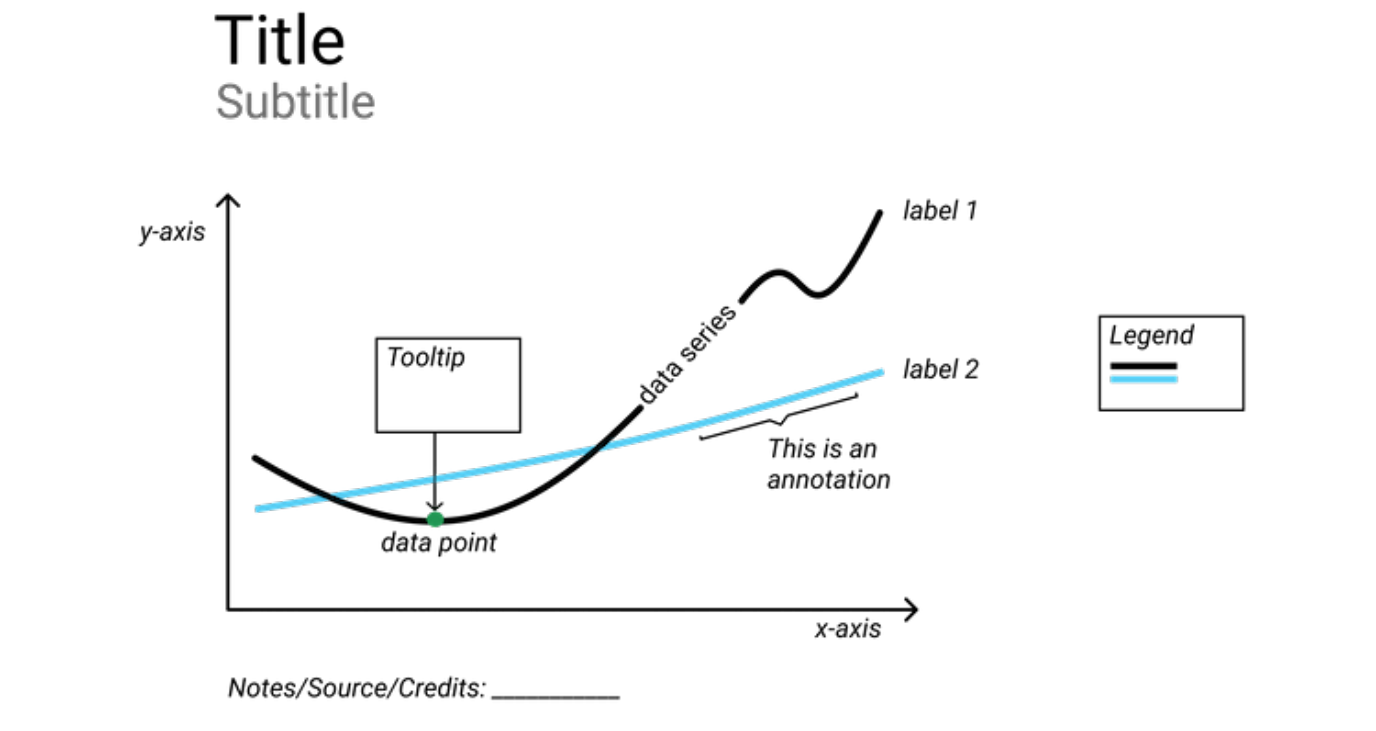
\includegraphics[width=\linewidth,height=.51\textheight,keepaspectratio]{images/part2_book/fig_6_1.png}\\[0.08cm]\figcaption{Các thành phần của biểu đồ}
\end{column}\end{columns}\takeaway{Thông tin cốt lõi phải hiện ra, không chỉ nằm trong hộp thông tin (tooltip).}
\note{Hãy xem hình như một bản hướng dẫn đọc dữ liệu: tiêu đề định hướng, trục và chú giải giúp giải mã. Những thông tin quan trọng phải hiện trực tiếp vì tooltip sẽ mất khi in hoặc trình chiếu ảnh tĩnh. Tiêu đề có thể kết hợp phụ đề ngắn về biến, địa điểm và thời gian. Nếu biết bất định, thể hiện thanh sai số khi phù hợp hoặc ghi hạn chế. Hình 6.1, trang 127. \url{https://handsondataviz.org/chart-design.html}}
\slidenumber{03}
\end{frame}

% ==================== SLIDE 4 ====================
\begin{frame}[plain,t]
\slideheader{Chương 6 • Chart Your Data}{Gốc 0 Phụ Thuộc Cách Mã Hóa}
\begin{columns}[T,onlytextwidth]
\begin{column}{.48\textwidth}
{\bodytext \textbf{Thanh / cột / miền}\\Độ dài hoặc diện tích thể hiện lượng. Giữ gốc 0 để tránh phóng đại chênh lệch.\par}\vspace{0.18cm}\centering 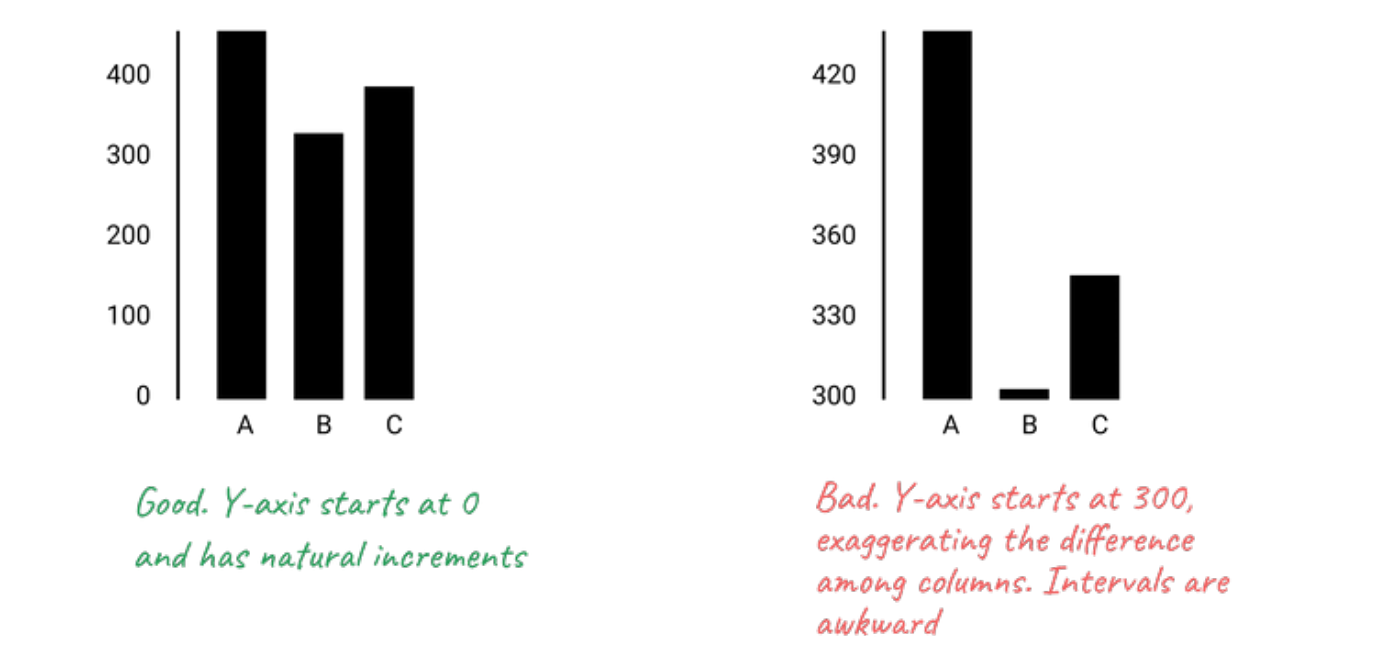
\includegraphics[width=\linewidth,height=.32\textheight,keepaspectratio]{images/part2_book/fig_6_2.png}\\[0.08cm]\figcaption{Cột: gốc 0 và trục bị cắt}
\end{column}
\begin{column}{.48\textwidth}
{\bodytext \textbf{Đường}\\Vị trí điểm thể hiện giá trị. Có thể thu hẹp trục để thấy thay đổi nhỏ.\par}\vspace{0.18cm}\centering 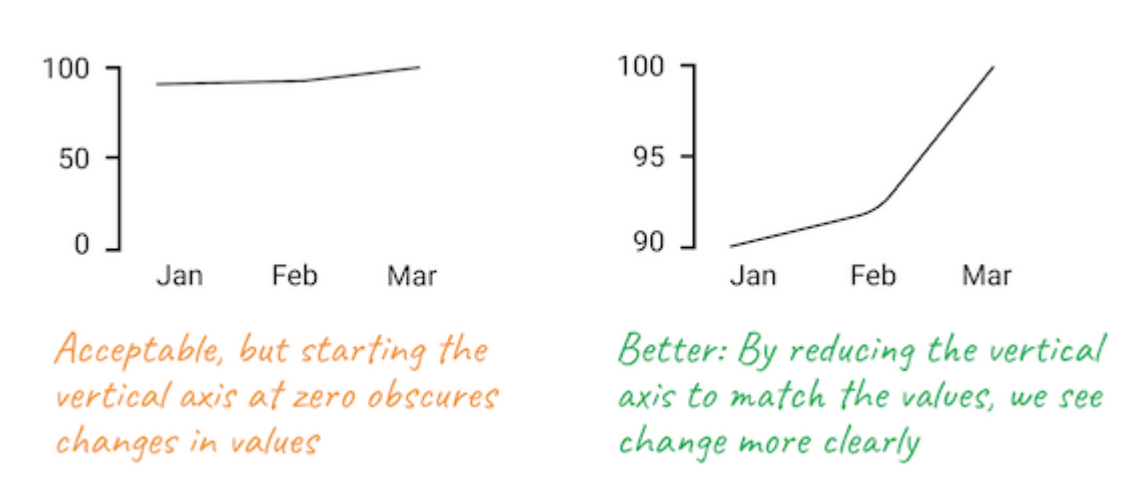
\includegraphics[width=\linewidth,height=.32\textheight,keepaspectratio]{images/part2_book/fig_6_4.png}\\[0.08cm]\figcaption{Đường: điều chỉnh khoảng trục}
\end{column}\end{columns}\takeaway{Trục đổi làm cảm giác chênh lệch đổi, dù dữ liệu giữ nguyên. Luôn đọc giới hạn trục.}
\note{Ở cột, người xem thường so độ dài nên cắt trục có thể làm khác biệt trông rất lớn. Với đường, trục không bắt đầu từ 0 vẫn có thể phù hợp; cần nhìn rõ giới hạn và đơn vị trước khi kết luận biến động mạnh hay nhẹ. Giữ gốc 0 cho thanh, cột và vùng tô diện tích. Trục đường từ 0 vẫn có thể chấp nhận. Hình 6.2 trang 128, hình 6.4 trang 130. \url{https://handsondataviz.org/chart-design.html}}
\slidenumber{04}
\end{frame}

% ==================== SLIDE 5 ====================
\begin{frame}[plain,t]
\slideheader{Chương 6 • Chart Your Data}{Biểu Đồ Tròn Thể Hiện Một Tổng 100\%}
{\bodytext Mỗi lát là một phần của \textbf{cùng tổng thể}. Các phần phải cộng thành 100\%.\par}\vspace{0.18cm}\begin{columns}[T,onlytextwidth]
\begin{column}{.48\textwidth}
\centering 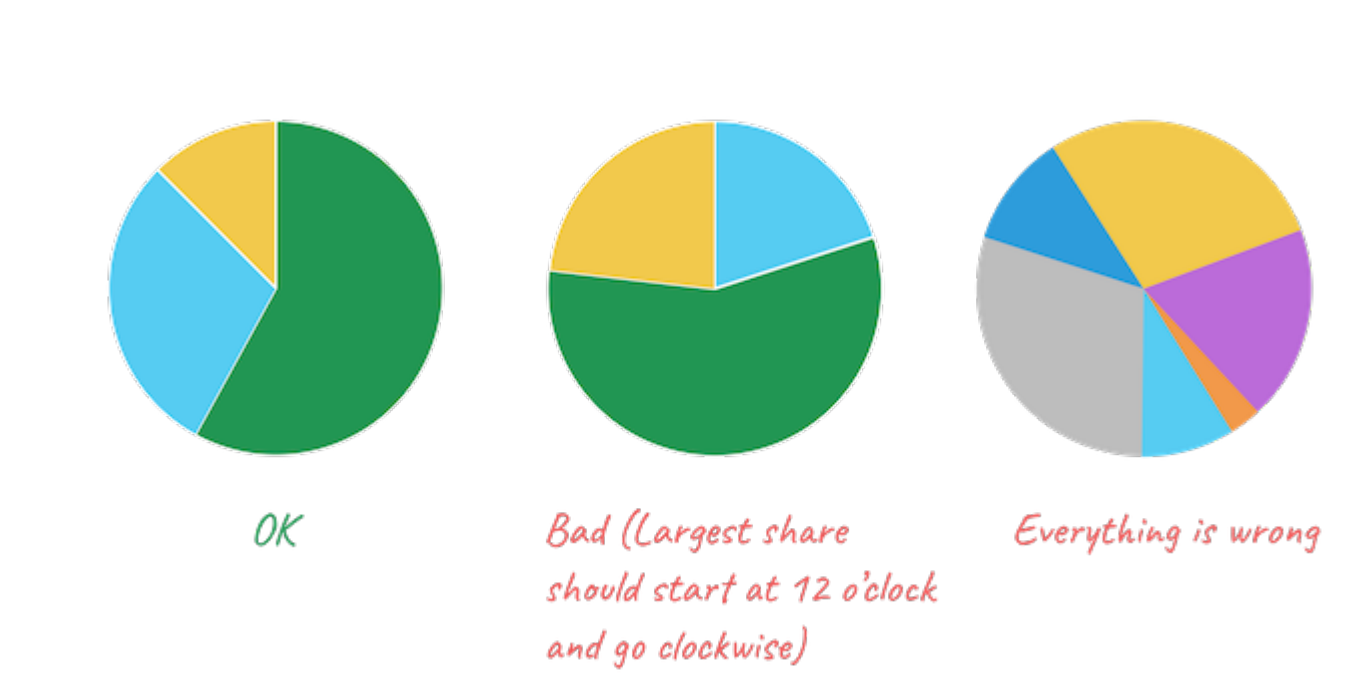
\includegraphics[width=\linewidth,height=.34\textheight,keepaspectratio]{images/part2_book/fig_6_6.png}\\[0.08cm]\figcaption{Câu hỏi cho chọn nhiều đáp án thường không phù hợp.}
\end{column}
\begin{column}{.48\textwidth}
\centering 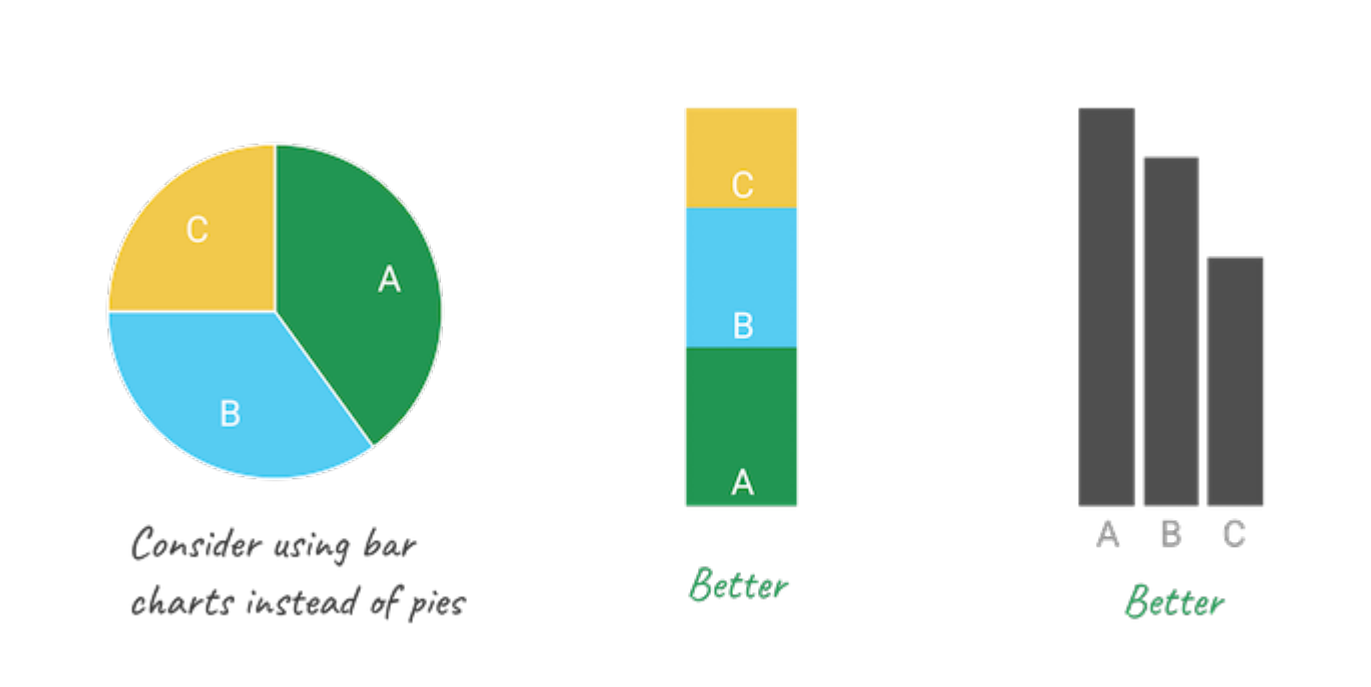
\includegraphics[width=\linewidth,height=.34\textheight,keepaspectratio]{images/part2_book/fig_6_7.png}\\[0.08cm]\figcaption{Các lát gần bằng nhau khó phân biệt. Thanh giúp so sánh rõ hơn.}
\end{column}\end{columns}\takeaway{Dùng ít lát và ghi nhãn rõ. Sách khuyến nghị không quá 5 lát.}
\note{Đọc biểu đồ tròn bằng cách đối chiếu từng phần với toàn bộ vòng tròn. Nếu mục tiêu là xếp hạng hoặc nhận ra chênh lệch nhỏ giữa các nhóm, biểu đồ thanh thường dễ đọc hơn. Sắp lát từ 12 giờ theo chiều kim đồng hồ là khuyến nghị về khả năng đọc của sách. Hình 6.6 trang 131, hình 6.7 trang 132. \url{https://handsondataviz.org/chart-design.html}}
\slidenumber{05}
\end{frame}

% ==================== SLIDE 6 ====================
\begin{frame}[plain,t]
\slideheader{Chương 6 • Chart Your Data}{Giữ Điều Giúp Người Xem Đọc Rõ}
{\bodytext \textbf{Rác đồ họa:} yếu tố trang trí làm giảm khả năng đọc.\par}\vspace{0.18cm}\begin{columns}[T,onlytextwidth]
\begin{column}{.30\textwidth}
\briefdef{Bỏ 3D, bóng đổ thừa}{Tránh làm méo cảm nhận.}
\briefdef{Nhãn dài: thanh ngang}{Tên nhóm dễ đọc hơn.}
\briefdef{Sắp xếp có lý do}{Theo giá trị hoặc thứ tự tự nhiên.}
\briefdef{Màu có mục đích}{Nhấn nhóm cần chú ý và dùng nhất quán.}
\end{column}
\begin{column}{.66\textwidth}
\centering 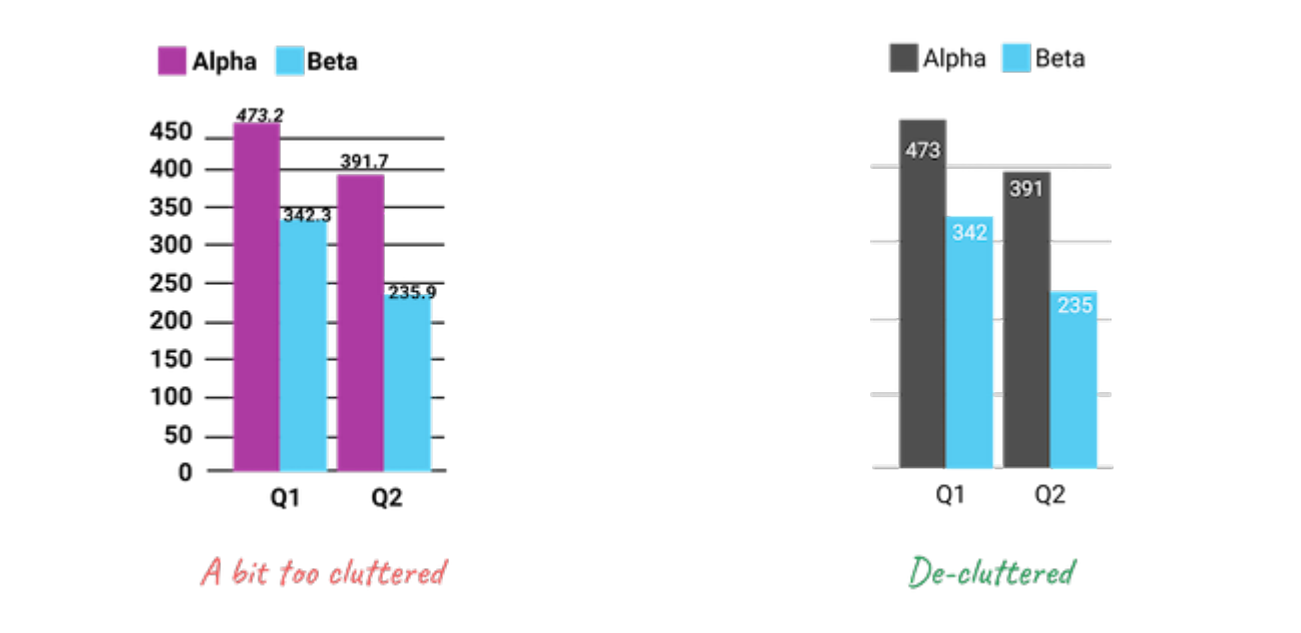
\includegraphics[width=\linewidth,height=.51\textheight,keepaspectratio]{images/part2_book/fig_6_11.png}\\[0.08cm]\figcaption{Tinh giản để làm rõ dữ liệu}
\end{column}\end{columns}\takeaway{Kiểm tra khả năng phân biệt màu và bản in trắng đen.}
\note{Trong hình, sự tinh giản giúp mắt tập trung vào độ dài và nhãn thay vì trang trí. Màu không nên là tín hiệu duy nhất: hãy kết hợp nhãn hoặc vị trí để người khó phân biệt màu vẫn theo dõi được. Tránh 3D giả tạo, không phải cấm biểu diễn dữ liệu thực sự ba chiều. Ý nghĩa màu phụ thuộc ngữ cảnh và văn hóa. Hình 6.11 trang 135. \url{https://handsondataviz.org/chart-design.html}}
\slidenumber{06}
\end{frame}

% ==================== SLIDE 7 ====================
\begin{frame}[plain,t]
\slideheader{Chương 6 • Chart Your Data}{Ba Cách So Sánh Danh Mục}
\begin{columns}[T,onlytextwidth]
\begin{column}{.315\textwidth}\begin{minipage}[t][2.0cm][t]{\linewidth}\raggedright\briefdef{Nhóm}{Đặt cạnh nhau để so nam và nữ trong từng nhóm tuổi.}\end{minipage}
\centering 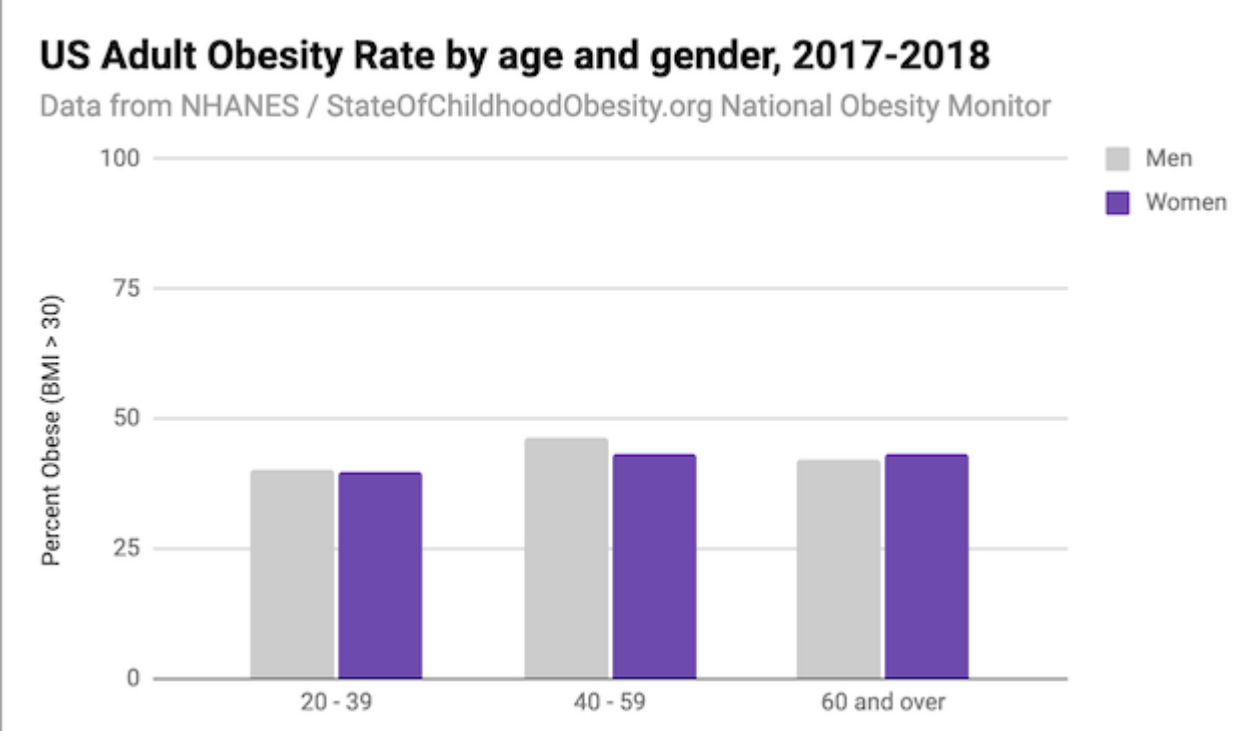
\includegraphics[width=\linewidth,height=.32\textheight,keepaspectratio]{images/part2_book/fig_6_13.png}\\[0.08cm]\figcaption{Béo phì theo tuổi / giới}\end{column}
\begin{column}{.315\textwidth}\begin{minipage}[t][2.0cm][t]{\linewidth}\raggedright\briefdef{Tách}{Chia cụm để đọc calo các món của từng nhà hàng.}\end{minipage}
\centering 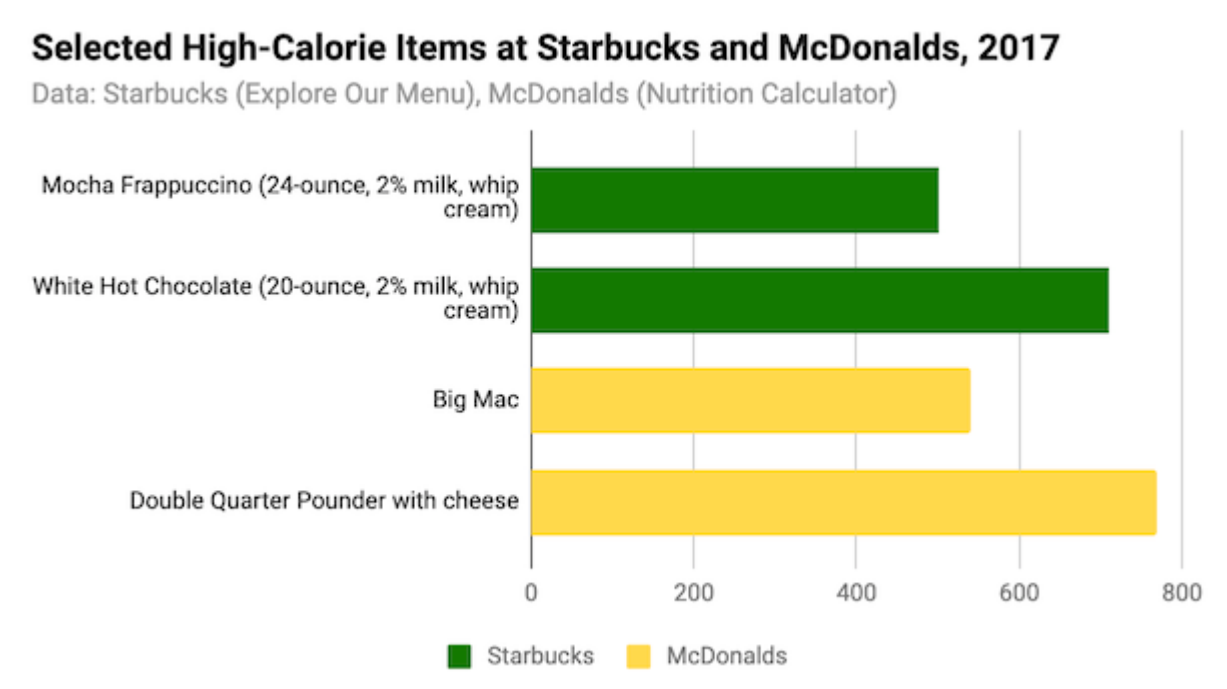
\includegraphics[width=\linewidth,height=.32\textheight,keepaspectratio]{images/part2_book/fig_6_23.png}\\[0.08cm]\figcaption{Calo món ăn theo nhà hàng}\end{column}
\begin{column}{.315\textwidth}\begin{minipage}[t][2.0cm][t]{\linewidth}\raggedright\briefdef{Chồng}{Đọc tỷ trọng các nhóm cân nặng trong mỗi quốc gia.}\end{minipage}
\centering 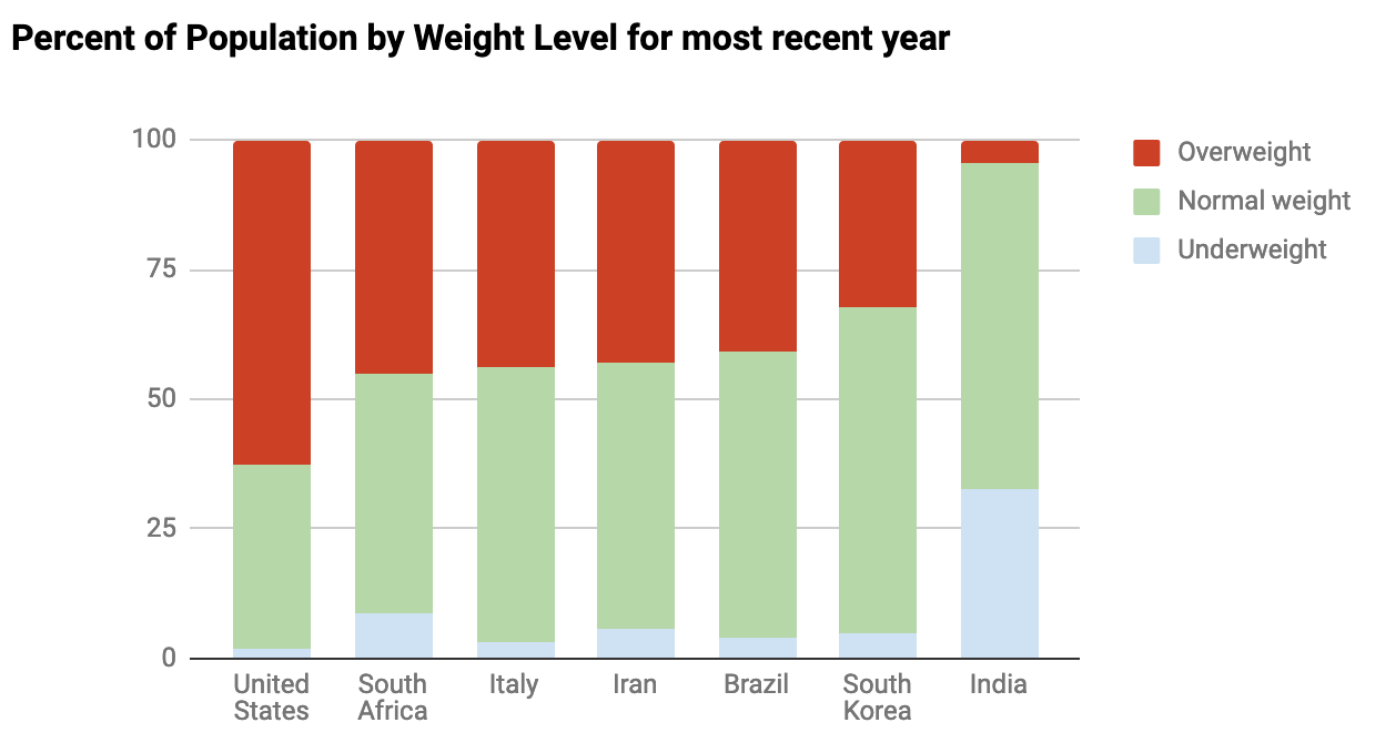
\includegraphics[width=\linewidth,height=.32\textheight,keepaspectratio]{images/part2_book/fig_6_25.png}\\[0.08cm]\figcaption{Nhóm cân nặng theo quốc gia}\end{column}
\end{columns}\takeaway{Nhóm và tách giúp so giá trị. Chồng giúp đọc thành phần trong tổng.}
\note{Không ghép từng món Starbucks với một món McDonalds thành các cặp tương ứng vì danh sách không giống nhau. Với cột chồng, phần ở đáy cùng gốc nên dễ so sánh hơn các phần ở phía trên. Hình 6.13 trang 137 dùng NHANES 2017--2018. Hình 6.23 trang 142 dùng thực đơn Starbucks và McDonalds. Hình 6.25 trang 144 dùng WHO và CDC. }
\slidenumber{07}
\end{frame}

% ==================== SLIDE 8 ====================
\begin{frame}[plain,t]
\slideheader{Chương 6 • Chart Your Data}{Histogram Cho Thấy Phân Bố}
{\bodytext Trục ngang là \textbf{khoảng calo (bin)}, trục dọc là \textbf{số quốc gia}. Các bin là khoảng số liên tiếp, thay vì danh mục.\par}\vspace{0.18cm}\begin{columns}[T,onlytextwidth]
\begin{column}{.30\textwidth}
{\bodytext\textbf{Cột cao:} nhiều quốc gia tập trung ở khoảng đó.\\[0.20cm]\textbf{Toàn dải:} mức phân tán và hai đuôi.\\[0.20cm]Đổi độ rộng bin có thể đổi hình dạng phân bố.\par}
\end{column}
\begin{column}{.66\textwidth}
\centering 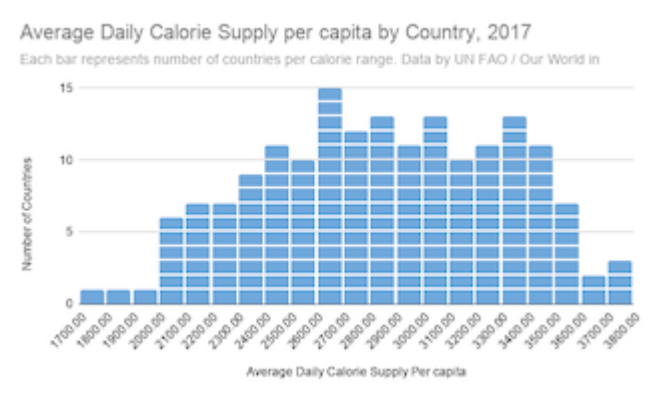
\includegraphics[width=\linewidth,height=.51\textheight,keepaspectratio]{images/part2_book/fig_6_28.png}\\[0.08cm]\figcaption{Nguồn cung calo/người/ngày • 174 quốc gia • 2017}
\end{column}\end{columns}\takeaway{Nguồn cung thực phẩm không đồng nghĩa lượng thực sự ăn.}
\note{Mỗi cột không đại diện một quốc gia mà đếm nhiều quốc gia trong cùng khoảng giá trị. Quan sát chỗ tập trung và hai đuôi giúp hiểu dữ liệu trước khi chọn cách chia nhóm hoặc làm bản đồ. Ví dụ FAO qua Our World in Data năm 2017 gồm 174 quốc gia. Đỉnh khoảng 2800 kcal. Không từ hình này gán nhãn đói nghèo hay dư thừa. Hình 6.28 trang 146. \url{https://handsondataviz.org/histogram-google.html}}
\slidenumber{08}
\end{frame}

% ==================== SLIDE 9 ====================
\begin{frame}[plain,t]
\slideheader{Chương 6 • Chart Your Data}{Đường Xem Từng Chuỗi, Miền Chồng Xem Tổng}
\begin{columns}[T,onlytextwidth]
\begin{column}{.48\textwidth}
{\bodytext \textbf{Đường:} theo dõi từng loại thịt và các giao cắt. Thịt gà tăng rõ ở giai đoạn cuối.\par}\vspace{0.18cm}\centering 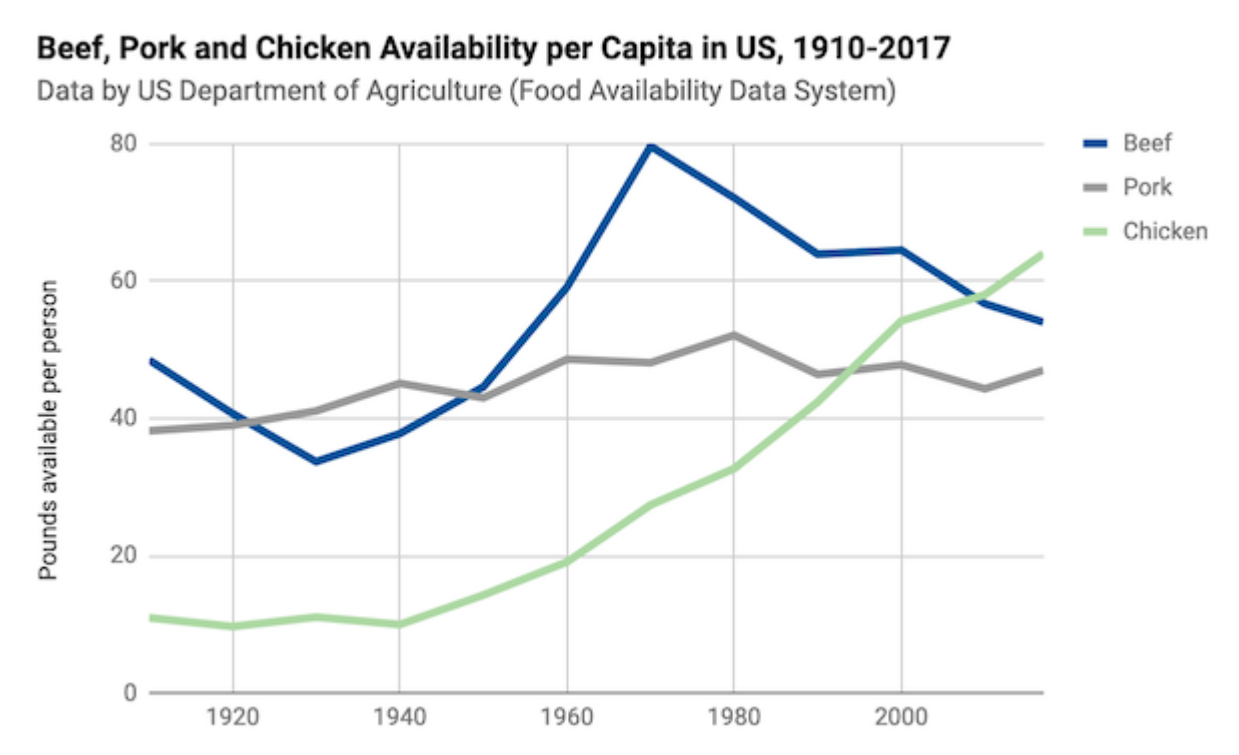
\includegraphics[width=\linewidth,height=.35\textheight,keepaspectratio]{images/part2_book/fig_6_33.png}\\[0.08cm]\figcaption{Dễ so sánh xu hướng của từng chuỗi.}
\end{column}
\begin{column}{.48\textwidth}
{\bodytext \textbf{Miền chồng:} độ dày mỗi dải là lượng từng loại. Biên trên cùng là tổng ba loại tại mỗi năm, không cộng dồn.\par}\vspace{0.18cm}\centering 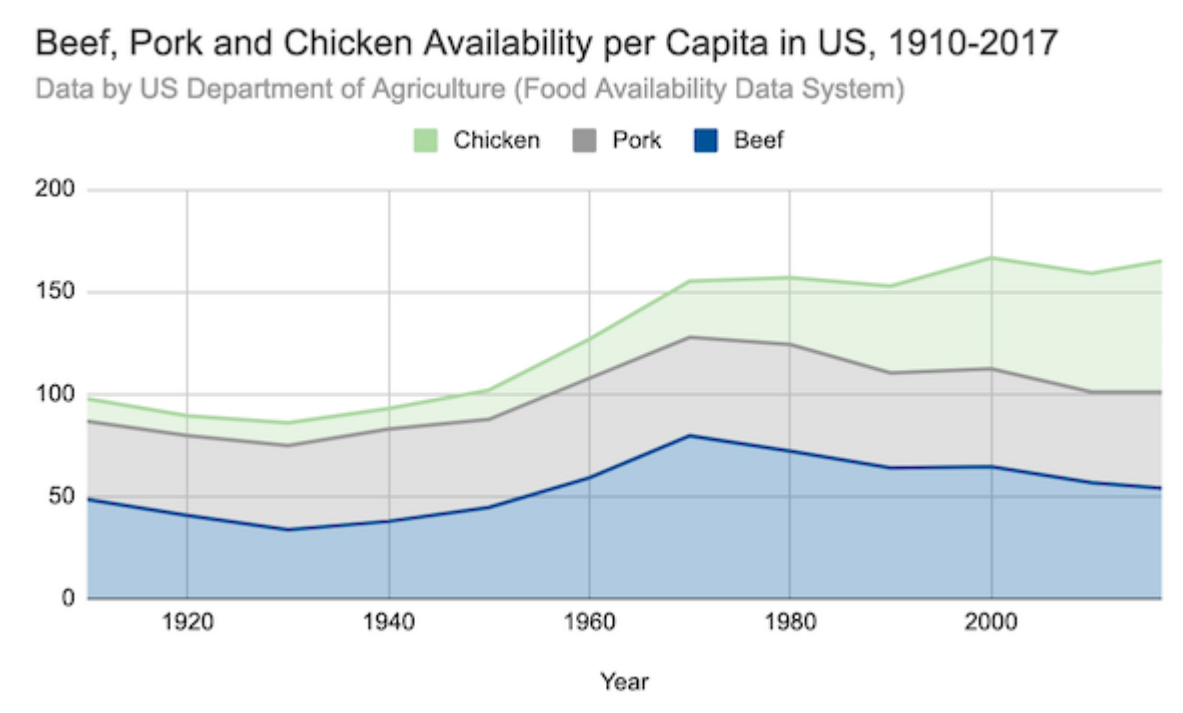
\includegraphics[width=\linewidth,height=.35\textheight,keepaspectratio]{images/part2_book/fig_6_34.png}\\[0.08cm]\figcaption{Tổng tại từng năm, không phải tổng cộng dồn.}
\end{column}\end{columns}\takeaway{Lượng thịt sẵn có bình quân đầu người tại Mỹ • USDA}
\note{Ở hình đường, ta dễ theo dõi một loại thịt từ đầu đến cuối. Ở miền chồng, đừng đọc đường biên trên của một dải thành giá trị riêng của loại đó: cần đọc độ dày dải; dữ liệu này cũng không đo lượng ăn thực tế. Miền thể hiện tổng ba loại tại từng năm, không cộng dồn qua các năm. Thịt gà vượt thịt bò và thịt lợn quanh năm 2000, không khẳng định chính xác năm nếu hình không chứng minh. Hình 6.33 trang 151 và 6.34 trang 152. \url{https://handsondataviz.org/pie-line-area-google.html}}
\slidenumber{09}
\end{frame}

% ==================== SLIDE 10 ====================
\begin{frame}[plain,t]
\slideheader{Chương 6 • Chart Your Data}{Range Làm Rõ Chênh Lệch}
{\bodytext Mỗi hàng là một bậc học. Hai điểm là \textbf{thu nhập trung vị của nam và nữ}. Đoạn nối càng dài, chênh lệch càng lớn.\par}\vspace{0.18cm}\centering 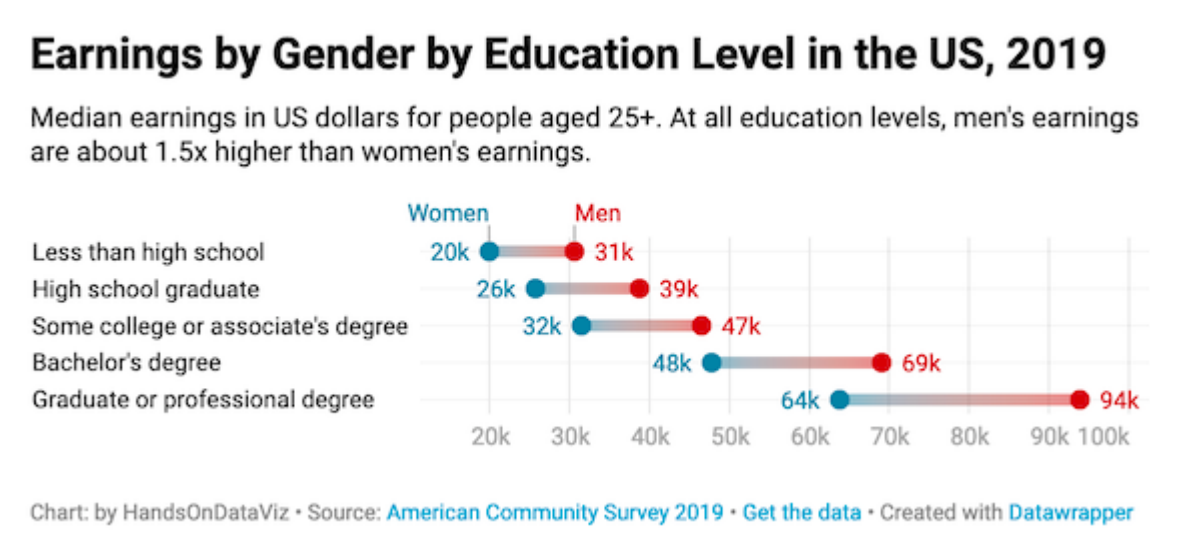
\includegraphics[width=.95\linewidth,height=.46\textheight,keepaspectratio]{images/part2_book/fig_6_39.png}\\[0.08cm]\figcaption{Thu nhập trung vị theo giới và học vấn • Người từ 25 tuổi trở lên • Mỹ, ACS 2019}\takeaway{Bậc cử nhân: nữ khoảng 48 nghìn USD, nam 69 nghìn USD.\\So sánh nhóm chưa cho biết nguyên nhân.}
\note{Mỗi hàng so sánh hai nhóm có cùng bậc học. Đoạn nối cho thấy mức chênh lệch trung vị, không mô tả mọi cá nhân và không xác định nguyên nhân. Ở bậc cử nhân, nữ khoảng 48 nghìn USD và nam khoảng 69 nghìn USD. Đây là thu nhập trung vị của người từ 25 tuổi trở lên trong ACS 2019, chưa điều chỉnh các yếu tố khác. Hình 6.39 trang 158. \url{https://handsondataviz.org/range-datawrapper.html}}
\slidenumber{10}
\end{frame}

% ==================== SLIDE 11 ====================
\begin{frame}[plain,t]
\slideheader{Chương 6 • Chart Your Data}{Phân Tán Cho Thấy Quan Hệ X–Y}
{\bodytext Mỗi điểm là một quốc gia. Vị trí kết hợp hai giá trị của \textbf{cùng quốc gia}.\par}\vspace{0.18cm}\begin{columns}[T,onlytextwidth]
\begin{column}{.30\textwidth}
\briefdef{X: tuổi thọ}{Sang phải là cao hơn.}
\briefdef{Y: số con / phụ nữ}{Lên trên là cao hơn.}
{\bodytext Tuổi thọ cao thường đi cùng số con thấp trong nhóm được chọn.\par}
\end{column}
\begin{column}{.66\textwidth}
\centering 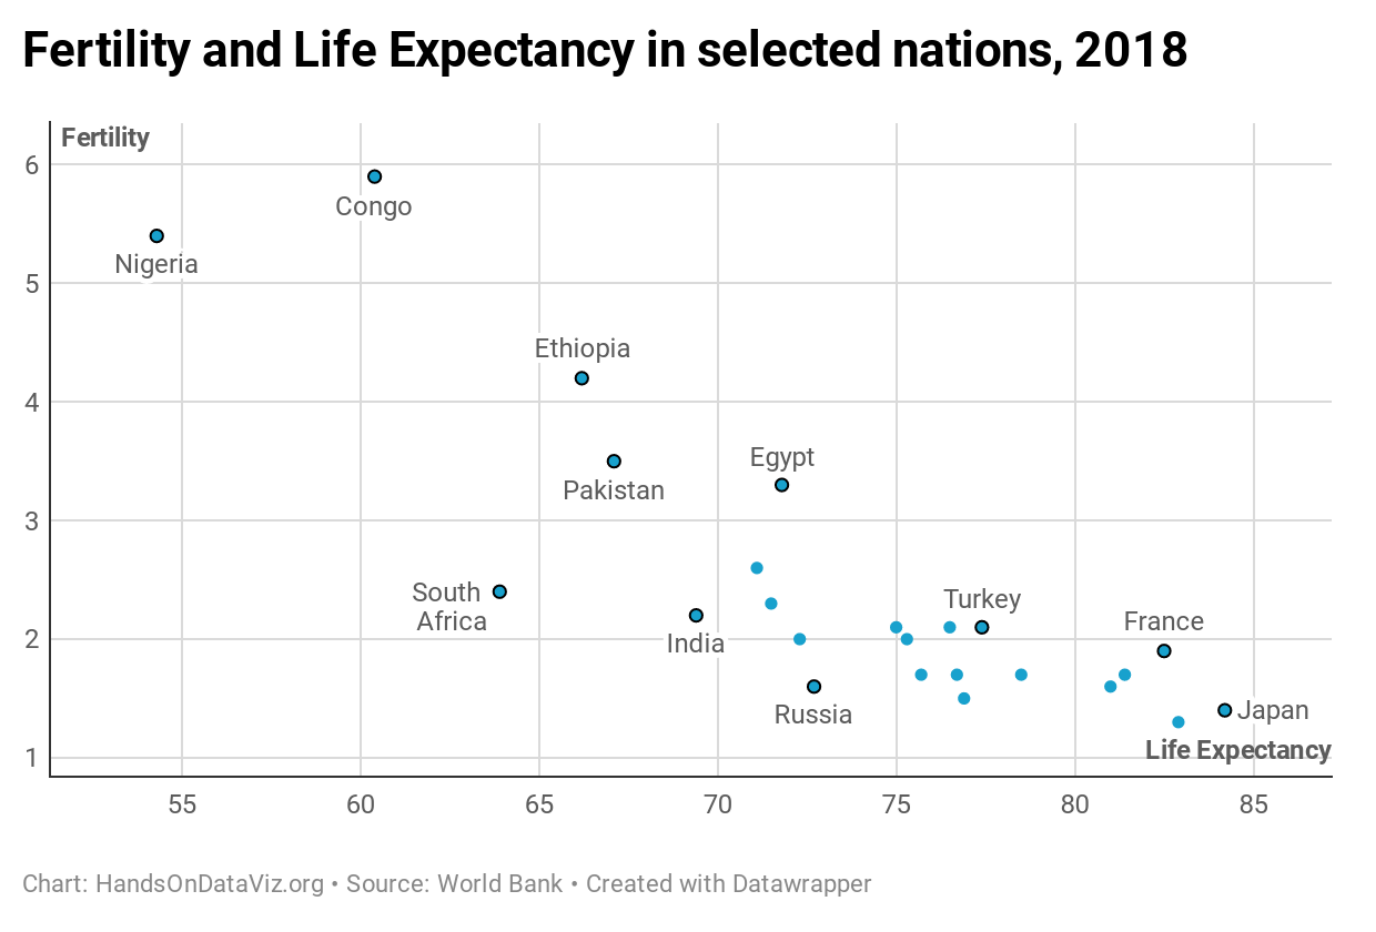
\includegraphics[width=\linewidth,height=.51\textheight,keepaspectratio]{images/part2_book/fig_6_44.png}\\[0.08cm]\figcaption{World Bank 2018 • Mỗi điểm là một quốc gia trong ví dụ}
\end{column}\end{columns}\takeaway{Tương quan không chứng minh nhân quả.}
\note{Ta đọc từng điểm bằng cả hai trục, rồi lùi lại để quan sát xu hướng chung và các điểm khác biệt. Không thể dùng hình này để kết luận sinh ít con làm tăng tuổi thọ hoặc ngược lại. Ví dụ dùng một số quốc gia được chọn trong World Bank 2018, không phải tất cả quốc gia. Số con trên một phụ nữ khác với số ca sinh trên nghìn dân. Hình 6.44 trang 162. \url{https://handsondataviz.org/scatter-bubble-datawrapper.html}}
\slidenumber{11}
\end{frame}

% ==================== SLIDE 12 ====================
\begin{frame}[plain,t]
\slideheader{Chương 6 • Chart Your Data}{Bong Bóng Thêm Kích Thước Và Màu}
{\bodytext Mở rộng biểu đồ phân tán bằng \textbf{hai biến nữa}.\par}\vspace{0.18cm}\begin{columns}[T,onlytextwidth]
\begin{column}{.30\textwidth}
\briefdef{X / Y:}{tuổi thọ và số con / phụ nữ.}
\briefdef{Diện tích bong bóng: dân số}{Bong bóng lớn hơn nghĩa là đông dân hơn.}
\briefdef{Màu: khu vực}{Các quốc gia cùng khu vực dùng cùng màu.}
\end{column}
\begin{column}{.66\textwidth}
\centering 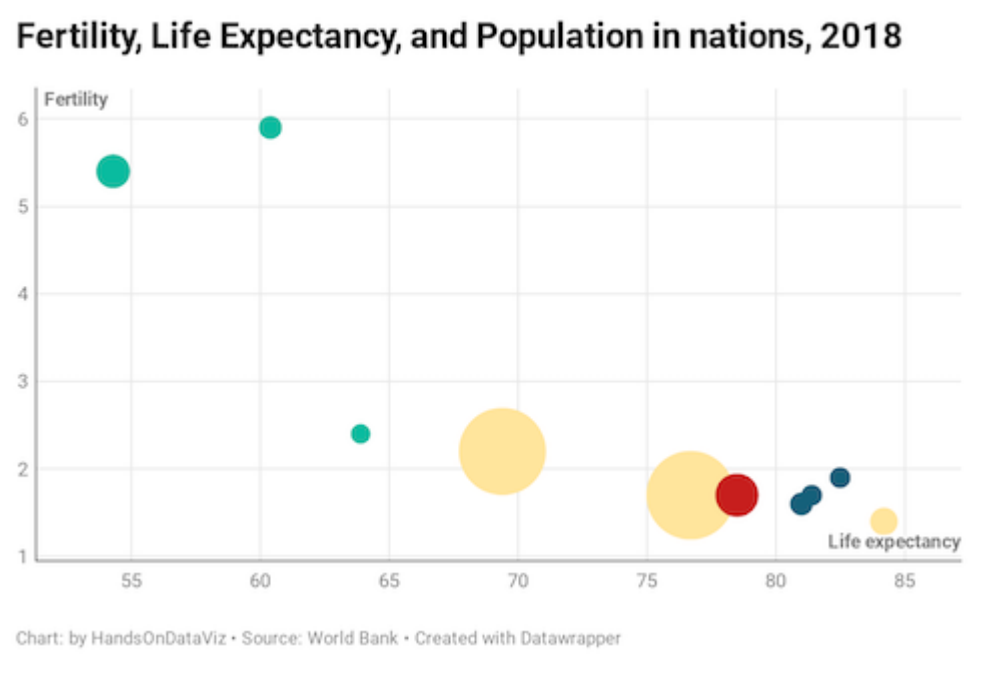
\includegraphics[width=\linewidth,height=.51\textheight,keepaspectratio]{images/part2_book/fig_6_48.png}\\[0.08cm]\figcaption{Tuổi thọ, số con/phụ nữ và dân số • World Bank 2018}
\end{column}\end{columns}\takeaway{Đọc kích thước theo diện tích, không theo bán kính. Chọn biểu đồ theo câu hỏi cần trả lời.}
\note{So với phân tán, bong bóng cho thêm bối cảnh về quy mô dân số và khu vực. Cần đọc kích thước theo diện tích, không theo bán kính; khi nhiều điểm chồng nhau, nhãn và công cụ tương tác có thể giúp tra cứu. Bốn biến qua X, Y, diện tích và màu. Tên quốc gia là định danh. Ví dụ tĩnh dùng các quốc gia được chọn trong World Bank 2018. Kết nối sang phần bản đồ bằng câu hỏi chọn hình thức biểu diễn phù hợp với dữ liệu. Hình 6.48 trang 165. \url{https://handsondataviz.org/scatter-bubble-datawrapper.html}}
\slidenumber{12}
\end{frame}

\end{document}
